\pdfoutput=1
\documentclass[11pt]{article}

\usepackage{acl}
\usepackage{times}
\usepackage{latexsym}
\usepackage[T1]{fontenc}
\usepackage[utf8]{inputenc}
\usepackage{microtype}
\usepackage{graphicx}
\usepackage{float}
\usepackage{titlesec}
\usepackage{tabularx}
\graphicspath{./images/}

\titlespacing*{\subsubsection}
{0pt}{5.5ex plus 1ex minus .2ex}{4.3ex plus .2ex}

\title{Playlist Generation using Emotion Recognition and Semantic Textual Similarity}

\author{
    Daniel King \\
    \And
    Thomas Hayter \\
}
\begin{document}
\maketitle


\section{Introduction}

The music scene has changed drastically over the last 20 years, and consumers have moved from listening either on the radio or via physical media to online streaming services such as Spotify \cite{streaming}. These streaming services deliver music in a variety of ways, one being the playlists that are generated for users to listen to. These playlists are accessible to all users and are shown to greatly improve the number of times those songs are streamed, which makes these playlists important to music artists wanting to spread their music. On top of this, streaming services want to attract as many customers to their service with the generation of playlists grouping similar songs together being one of their selling points.

\begin{figure}[H]
    \centering
    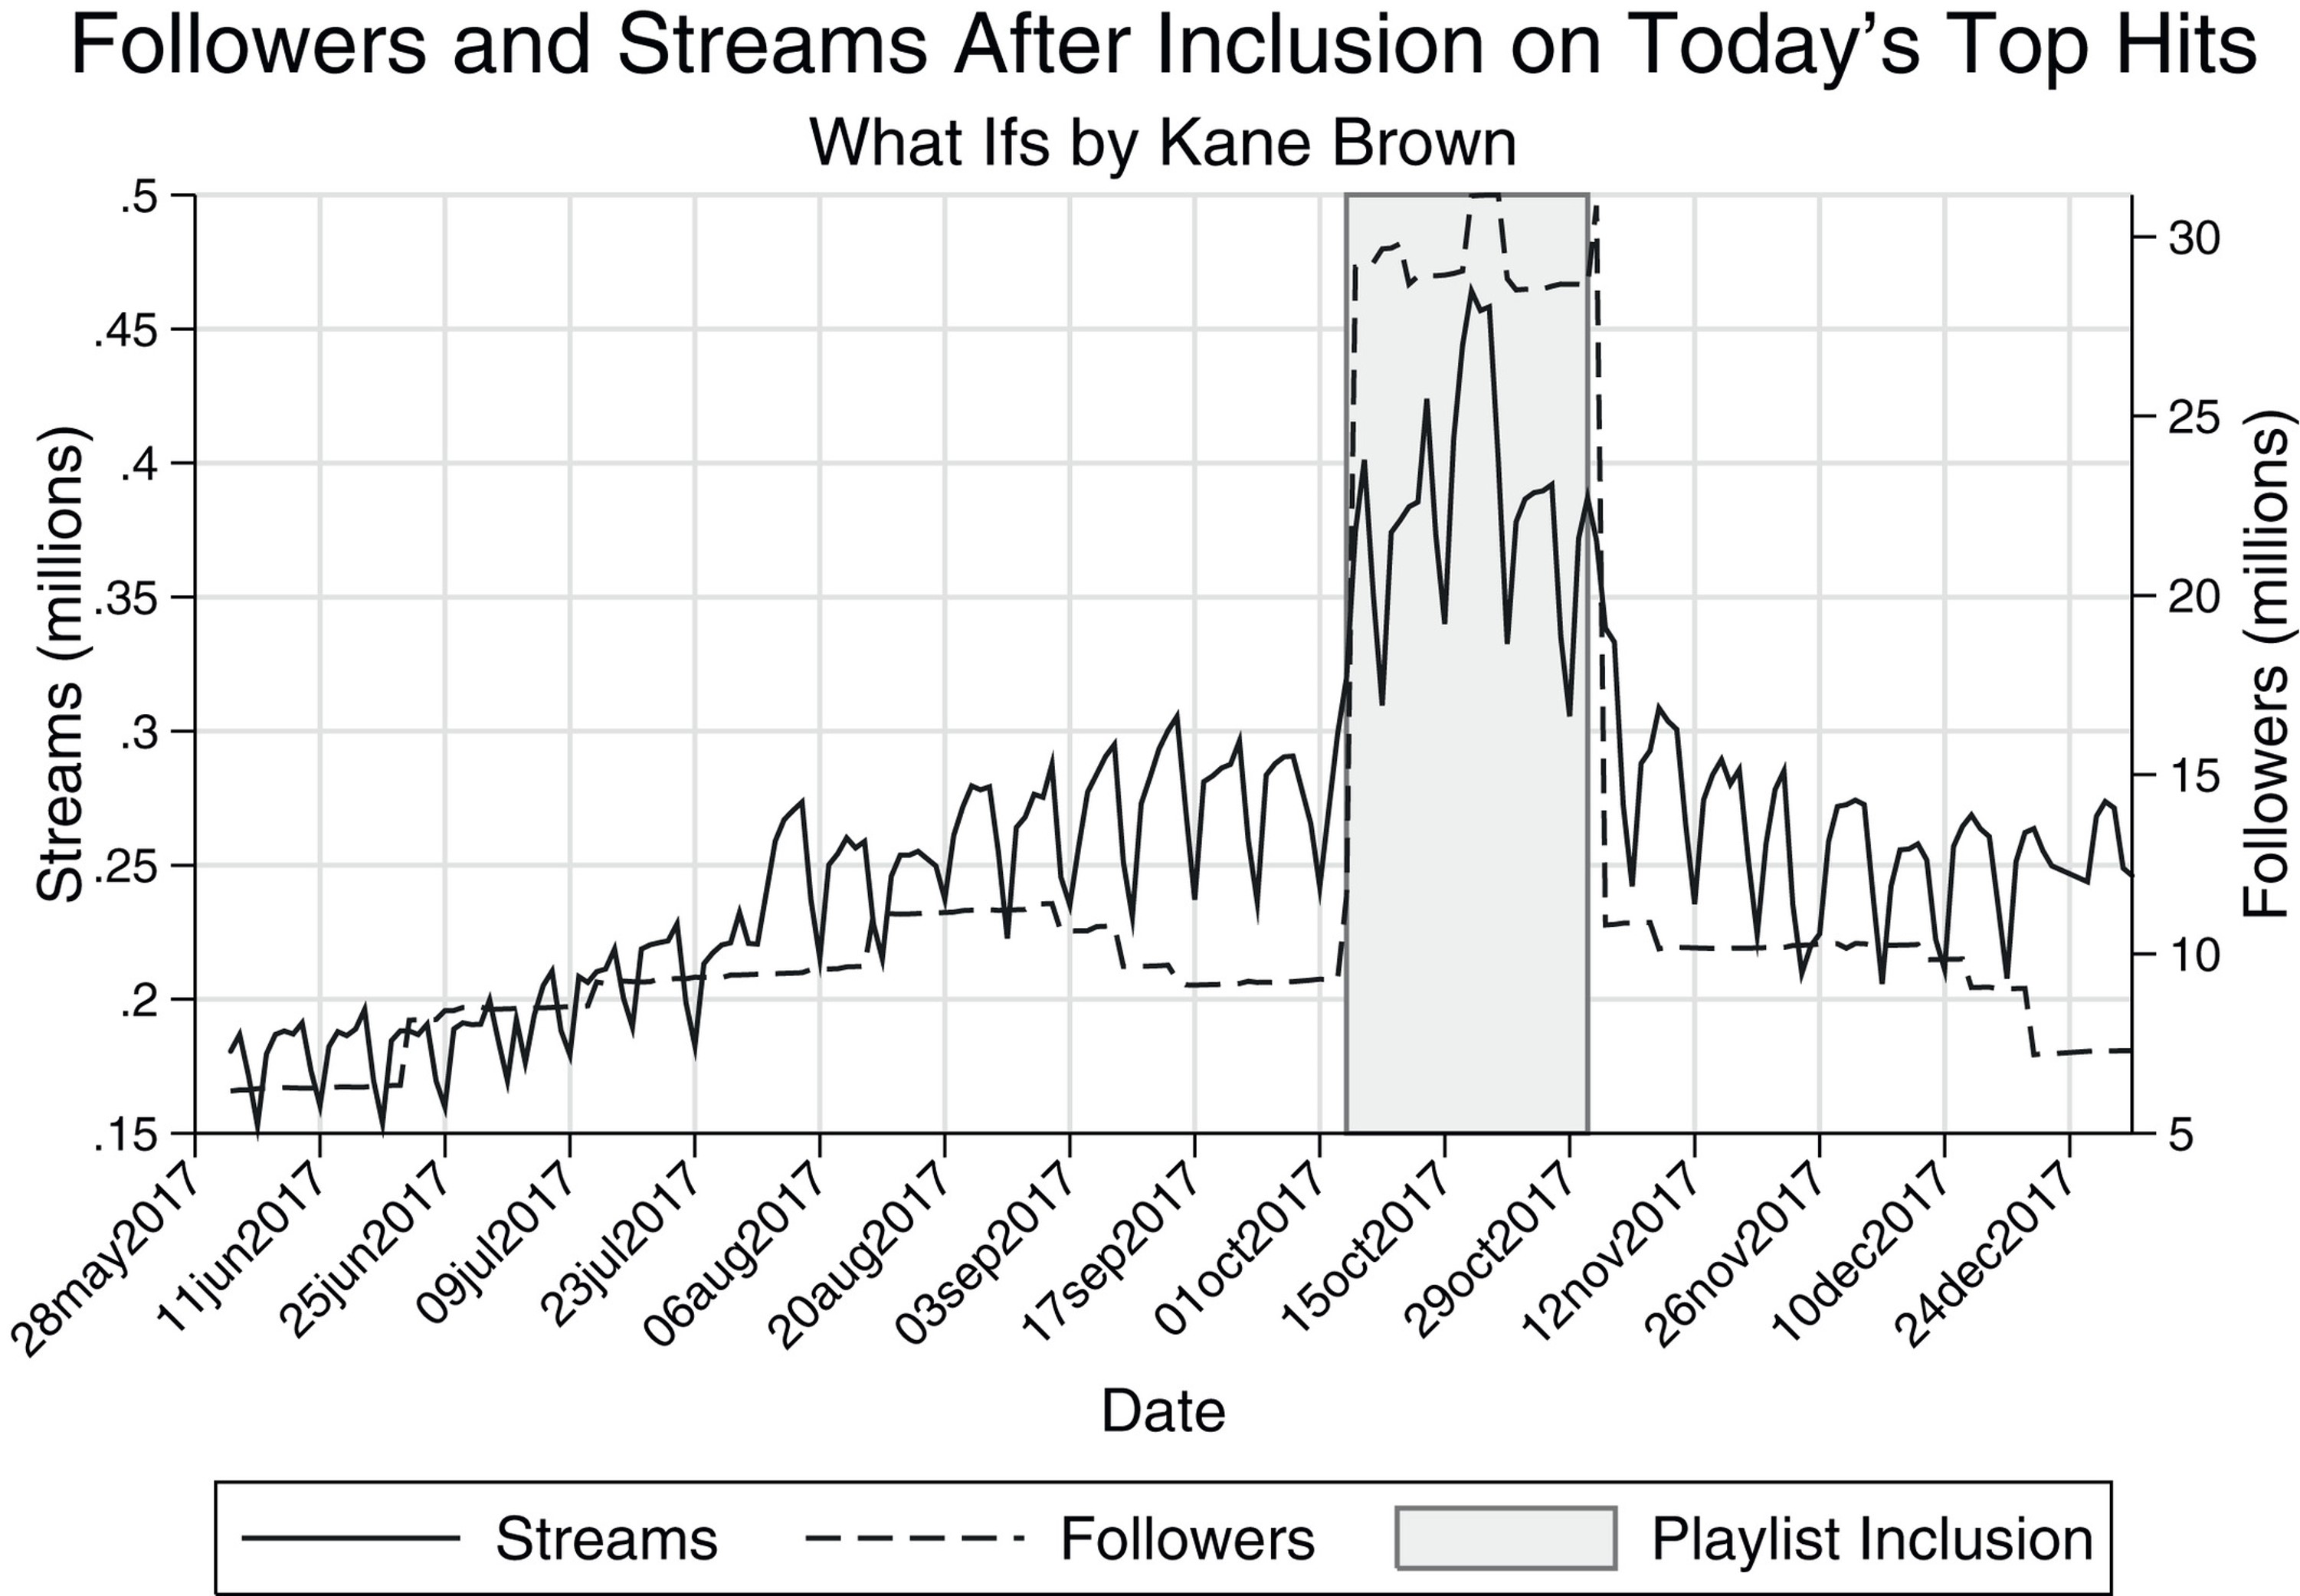
\includegraphics[width=0.48\textwidth]{images/PlaylistStreams.jpg}
    \caption{Graph showing the followers and streams on inclusion in Spotify's playlist Today's Top Hits. Taken from \cite{playlists}}
\end{figure}

This discusses a novel system for playlist generation, taking an input text and producing a list of songs with similar emotions and semantic meanings within their lyrics. 

\section{Related Work}

Emotion recognition (ER) is the task of assigning emotions to an input, in this case song lyrics. It can be applied to many different fields, such as natural language processing, human-computer interaction and psychology \cite{emotionRecognition}. Multiple approaches exist to the task exist, such as rule-based, classical learning and deep learning methods. Pre-trained models, for example BERT \cite{bert}, have seen success classifying multiple emotions within song lyrics \cite{edmonds-sedoc-2021-multi}.

Semantic textual similarity (STS) is the task of comparing two texts and deciding whether they have similar meaning. There are many approaches to this task, such as comparing vector embeddings, comparing alignment and using machine learning models \cite{semanticTextSimilarity}. After producing word vectors with GloVe \cite{pennington-etal-2014-glove}, Sanborn et al. evaluated using both recurrent and recursive neural networks to calculate semantic similarity \cite{Sanborn2015DeepLF}.

\section{Methodology}
The methodology of the project can be split up into different steps, which can be seen in the flowchart below. Each of the different steps will be explored in detail.

\begin{figure}[H]
    \centering
    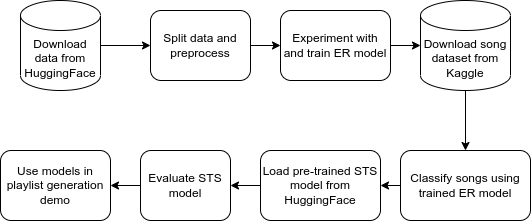
\includegraphics[width=0.48\textwidth]{images/codeFlow.png}
    \caption{Flow chart showing the steps of the project}
\end{figure}

\subsection{Emotion Recognition Model}
The first task to be performed was to train an emotion recognition model to classify a given input of text into an emotion class. The dataset used was the dair-ai/emotion dataset \cite{emotiondata} from HuggingFace. The dataset consists sentences that have been classified into one of six separate emotion classes - sadness, joy, love, anger, fear and surprise. The dataset contains two separate splits; one with 20,000 samples split into a training, testing and validation set, and another with 417,000 samples in one set. For this project, the larger split with 417,000 samples was chosen to train the model.

After being read in, the dataset was checked for imbalances between the labels in the dataset, which was immediately obviously present. The sadness and joy classes had 121,187 and 141,067 samples respectively, while the surprise class only had 14,972 samples. To combat this imbalance, downsampling was performed to randomly select 5,000 samples from each of the classes to form a new dataset of 30,000 samples. Due to a lack of dedicated hardware to quickly train models, a smaller dataset of only 2,000 samples was created using the same downsampling method - to be used for experimenting with hyperparameters before training the final model. The larger dataset was split into a training and testing set, with a 0.85:0.15 train:test split; resulting in 25,500 samples being used for training and 4,500 for testing. The smaller dataset was also split.

The approach decided upon to create the model was to fine-tune a pre-trained BERT \cite{bert} model, by minimising cross entropy loss on the predictions of the classes. This was done using PyTorch and transformers. To preprocess the data, all of the data was encoded using the BertTokeniser, which tokenised the data. It then returned both the input ids of all of the tokens, as well as the attention mask for the given input, so that padded values could be ignored (padding was used to ensure all inputs were of the same length). Before tuning the final model, an experiment was run with different model parameters to see which gave the best performance, and this experimentation will be discussed in more detail in the evaluation section. Using the best found parameters, the model was then fine-tuned on the larger training set by minimising cross entropy loss. To speed up the training process, Adam optimiser was used when training. The model returns logits, so an argmax function was used to get the predicted class from the output of the model. Metrics such as the precision, recall and f1 score across the different classes were calculated. The final trained model was then saved using PyTorch to be loaded in later when making predictions.

\subsubsection{Generating Song-Emotion Dataset}
To have songs to generate playlists from, the Spotify Million song dataset \cite{spotify} from kaggle was used. The dataset consists of songs with the artist, song title, a link to the song and song lyrics. To create the emotion-song dataset, the lyrics of the songs were first cleaned to remove newline characters, then passed into the trained emotion recognition model. The logits from the output of the model were taken, and any class with positive logits returned was said to be an emotion 'present' in the current song lyrics. Using this output of the emotion classes for each song, a dictionary of emotions mapping to a list of indices of the songs containing the emotions was constructed to be used alongside the song dataset in the final demo.

\subsection{STS Model}

To calculate the semantic textual similarity between two songs, a MiniLM \cite{minilm} model, which is a distilled version of a large transformer model such as BERT \cite{bert}, was used. The particular model in question had 6 layers, was fine-tuned on a dataset of 1B sentence pairs, and was loaded from HuggingFace \cite{stsmodel} using sentence-transformers. To compare the similarity between embeddings generated by this model, a function to compute cosine similarity was written and used. All pre-processing/encoding needed was performed by the model itself, so no such code was necessary when using this model. 
An experiment to evaluate the performance of this model was written and run, but shall be discussed in the evaluation section of this report.

\subsection{Demo}
\begin{figure}[H]
    \centering
    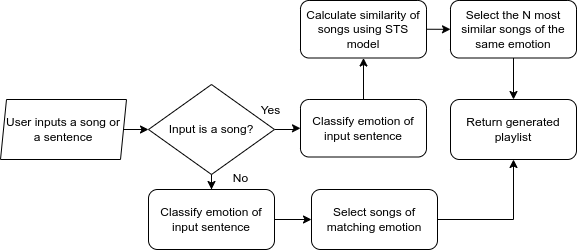
\includegraphics[width=0.48\textwidth]{images/DemoFlow.png}
    \caption{Flow chart showing the program flow of the demo}
    \label{fig:flow}
\end{figure}

The flow chart in Figure \ref{fig:flow} depicts the code flow of the final demo notebook. Both the ER model and the STS model are loaded into the notebook, as well as the song dataset and the song-emotion dictionary. The user is allowed to generate playlists in two different ways. First, they can enter an input sentence, which will have its emotion detected by the ER model, and then a playlist, of length defined by the user, with songs of the same emotion as the input sentence will be generated. The second option is to input song lyrics. In this option, the emotion of the song is detected and songs from the same emotion are selected as candidates for the playlist. Then, the STS model calculates the similarity between the input lyrics and the songs in the database, and the top N most similar songs are selected to be put into the playlist - where N is the length of the playlist defined by the user.

\section{Evaluation}

\subsection{ER Model}

When experimenting with the performance of the ER model, the factors to consider were the learning rate of the model, and how many epochs of training to do. To find the optimal values of these parameters, a grid search was performed using 3 learning rate values of 1e-3, 1e-4, and 1e-5 and 3 epoch numbers of 10, 20, and 30. The data was trained on the training set and the loss on the testing set measured at each of the epoch values. By increasing the number of epochs, and using a low learning rate, we expect the model to perform better as it would allow for the best fit onto the training data. However, if this doesn't result in the best performance, it is most likely due to the fact that the model has overfit on the training data and so performs worse on the training data. The results of the experiment can be seen in Table \ref{tbl:crossEntropy}.

\begin{table}[H]
    \centering
    \caption{A table showing the Cross Entropy loss of the model with different hyperparameter values}
    \begin{tabularx}{0.48\textwidth}{|X X X|} 
      \hline
      \multicolumn{3}{|c|}{Learning rate 1e-3} \\ \hline 
      10 epochs & 20 epochs & 30 epochs \\ \hline
      $1.91$&$1.84$ &$1.79$ \\ \hline
    \end{tabularx}
    \begin{tabularx}{0.48\textwidth}{|X X X|} 
        \hline
        \multicolumn{3}{|c|}{Learning rate 1e-4} \\ \hline 
        10 epochs & 20 epochs & 30 epochs \\ \hline
        $0.83$&$0.94$ &$1.04$ \\ \hline
      \end{tabularx}
      \begin{tabularx}{0.48\textwidth}{|X X X|} 
        \hline
        \multicolumn{3}{|c|}{Learning rate 1e-5} \\ \hline 
        10 epochs & 20 epochs & 30 epochs \\ \hline
        $0.41$&$0.48$ &$0.48$ \\ \hline
    \end{tabularx}
    \label{tbl:crossEntropy}
\end{table}

From this table, we can see that reducing the learning rate did greatly increase performance. With a high learning rate of 1e-3, the weight updates are too large and the model fails to converge onto a well performing weight settings. In contrast, with a much lower learning rate of 1e-5, the model quickly converges on a good performing set of weights. Unlike what we expected, the model actually performs better with a lower number of epochs, with 10 epochs being the best performing settings. We believe this is because at the larger number of epochs, the model overfit on the training data and thus didn't perform as well when shown unseen data.

\subsection{STS Model}


To evaluate the performance of the STS model on song data, a custom testing metric was written. Taking a random song from a given emotion class, two other songs were selected - one from the same emotion class, and another from a random differing emotion class. A prediction is considered 'correct' if the model marks the song from the same emotion class as more similar than the song from the different emotion class.
We expect the number of correctly classified songs to be at least 60\%, as it shows that the model is definitely classifying songs of the same emotions as more similar. However, if this doesn't come to pass, it is hard to say whether it is due to the performance of the model, or the fact that two songs from the same emotion class aren't necessarily more textually similar.

\begin{table}[H]
    \centering
    \caption{A table showing the \% accuracy of the STS model across 3 runs of the experiment}
    \begin{tabularx}{0.48\textwidth}{|X X X|} 
      \hline
      \multicolumn{3}{|c|}{Accuracy} \\ \hline 
      Repeat 1 & Repeat 2 & Repeat 3 \\ \hline
      $0.57$&$0.78$ &$0.6$ \\ \hline
    \end{tabularx}
    \label{tbl:stsAcc}
\end{table}

Table \ref{tbl:stsAcc} shows the results of the experiment across 3 iterations. The average accuracy across the 3 iterations is 65\%, which is promising accuracy. However, due to the large standard deviation of 9.3\%, and a range of 21\% across the 3 iterations, it is fair to say that this is quite an unreliable metric of accuracy for the model. This unreliability is most likely due to the fact that songs from different emotion classes can still be textually similar, which greatly skews the performance of the metric.

\subsection{Playlist Generation}

There is no mathematical way to evaluate the performance of the final playlist generation, as the performance is subjective. However, in future, it would be possible to run some form of user testing, where users marked songs selected in the generated playlist as appropriate or inappropriate, and some form of performance metric could be calculated based on the percentage of appropriate songs that the system selects.

\section{Discussion}

We have trained an emotion recognition model and, combined with a semantic embedding model, developed a playlist generation system that produces a playlist of songs emotionally and semantically similar to an input text. At first glance, the system appears to perform well. The playlists generated contain songs that are all focused around the same topics as those in the input text.

\begin{table}[h]
    \centering
    \caption{A table showing the precision, recall and f1 scores for each emotion recognised by the emotion recognition model}
    \begin{tabularx}{0.48\textwidth}{| X | X X X |} 
      \hline
      Emotion & Precision & Recall & f1 score\\ \hline
      sadness & $1.00$ & $0.96$ & $0.98$ \\ 
      joy & $0.96$ & $0.97$ & $0.96$ \\ 
      love & $0.98$ & $0.98$ & $0.98$ \\ 
      anger & $0.93$ & $1.00$ & $0.97$ \\ 
      fear & $0.89$ & $0.91$ & $0.90$ \\ 
      surprise & $0.95$ & $0.86$ & $0.90$ \\ \hline
    \end{tabularx}
    \label{tbl:f1}
\end{table}

The results in Table \ref{tbl:f1} show that the emotion recognition model performed very well overall. Fear and surprise were the two emotions that the model struggled with the most, however even then the model was achieving an f1 score of 0.9. While this performs better than the model produced by Edmonds et al. \cite{edmonds-sedoc-2021-multi}, it is tested using a dataset of tweets rather than a dataset of song lyrics due to the lack of available data. Therefore, the same performance can not be guaranteed when recognising emotions in songs.


\begin{figure}[H]
    \centering
    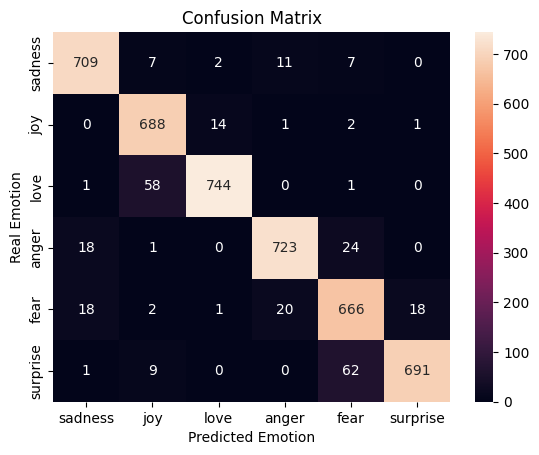
\includegraphics[width=0.48\textwidth]{images/Confusion.png}
    \caption{Confusion matrix for the emotion recognition model}
    \label{fig:confusion}
\end{figure}

Figure \ref{fig:confusion} shows the confusion matrix for the emotion recognition model, which was generated to assess the model by each emotion it detects. The incorrectly labelled tweets were still generally labelled with similar emotions. For example, 58 tweets labelled love were predicted joy, however it can be argued that these two emotions are similar and often come hand in hand. This is reassuring, as the model is not drastically wrong when it is incorrectly labelling songs. Therefore, there will not be many glaring errors when producing a playlist of songs with the same emotion. 



\section{Conclusion}

A playlist generator has been produced that takes an input text, and produces a list of N songs that have emotionally and semantically similar lyrics. This can be used by streaming services and their users to generate new playlists with new songs.

This project could be continued by connecting this system to a user interface that allows a user to select an existing song or enter input text in a more user-friendly environment. It could also be linked to the Application Programming Interface (API) for a streaming service to actually produce these playlists within the service.

\bibliographystyle{acl_natbib}
\bibliography{custom}


\end{document}
